\chapter{软件实现与测试}

\section{软件界面展示与功能测试}

1、测试环境
2、测试用例
3、测试结果

\section{果实图像识别模型的训练}

农业果实称重云端软件基于 YOLOv8 实现果实图像识别功能,训练数据集来源于 Kaggle 平台上的已经完成数据标注的 Fruits-360 数据集。训练流程如下:

1、挑选来自 22 种不同果实的近三千张照片,将其上传至 roboflow 平台;

2、在 Kaggle 云平台上,通过 roboflow 提供的 API,将数据导出为 YOLOv8 格式的数据集;

3、使用 YOLOv8 模型训练数据集。训练进行 50 个 epoch,使用 yolov8m 预训练模型作为基础。训练过程中,如果验证集的性能在 30 个 epoch 内没有改进,训练将提前停止。

模型训练完成后,得到标准化混淆矩阵图如下:

\begin{figure}[H]
    \centering
    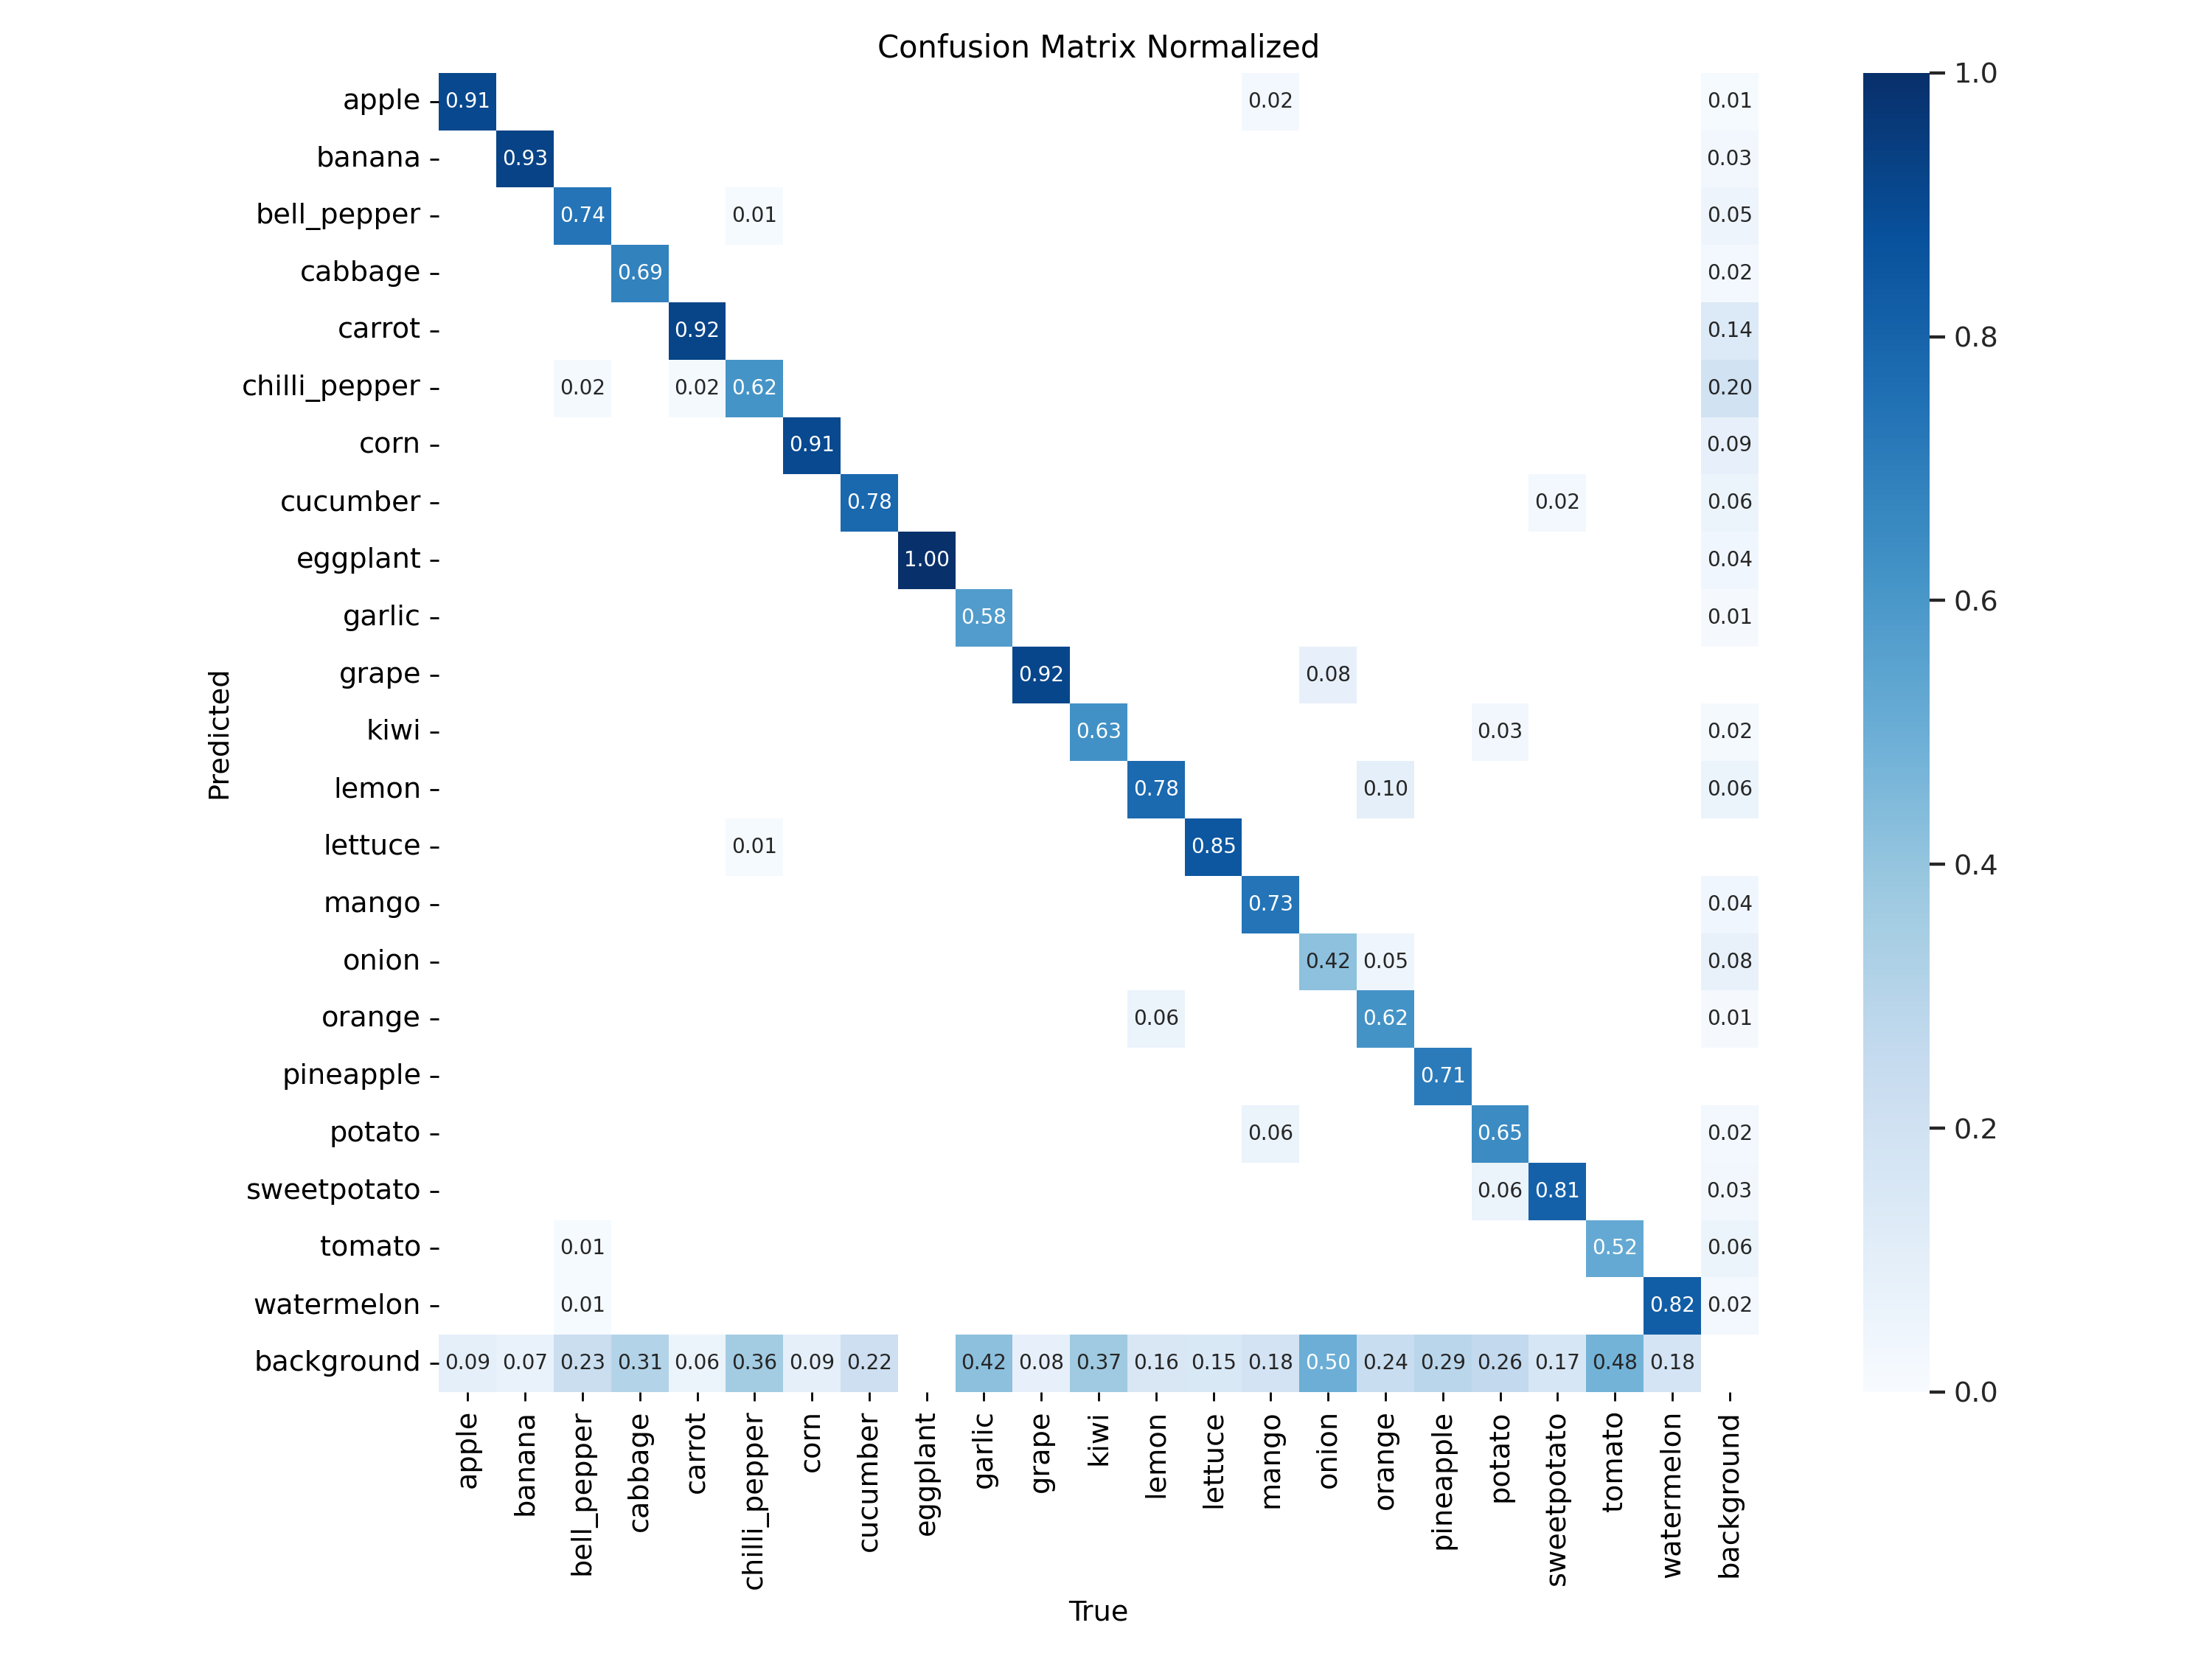
\includegraphics[width=0.8\linewidth]{../source/aws-img/yolov8/out/image/confusion_matrix_normalized.png}
    \caption{果实图像识别模型训练结果-标准化混淆矩阵图}
    \label{fig:confusion_matrix_normalized}
\end{figure}

从图中的标准化混淆矩阵可以看出,模型在多个类别上表现出色。例如,apple、banana 和 carrot 等类别的预测准确率都超过了 90\%,表明模型在这些类别上的预测非常精确。具体来说,apple 的准确率为 91\%,banana 为 93\%,而 carrot 为 92\%。

然而,某些类别的分类效果较差,尤其是在 chilli\_pepper 和 background 类别上。chilli\_pepper 的准确率为 62\%,并且容易被误分类为 corn 或其他类别。此外,模型在识别 background 类别时的准确率较低,为 18\%,这可能是由于背景图像的多样性和噪声所致。

总体来说,模型在多数类别上的表现良好,但对于某些类别的混淆仍然存在,尤其是那些外观相似的类别(如 bell\_pepper 和 cabbage)。这种混淆可能来源于数据集中的样本不均衡、类别相似性较高或特征不足等问题。


1、测试环境
2、测试用例
3、测试结果

\section{针对核心接口的性能测试}

1、测试环境
2、测试用例
3、测试结果

\section{本章小结}